While additional cores and newer architectures, such as those provided
by GPU clusters, steadily increase available compute power, memory
and disk access has not kept pace, and most believe this trend will
continue.  It is therefore of critical importance that we design
systems and algorithms which make effective use of off-processor
storage.  This work details our experiences using parallel file
systems, details performance using current systems and software,
and suggests a new API which has greater potential for increased
scalability.

\section{Introduction}

Large scale parallelism is widely used not only to simulate complex
phenomenon, but also to process the resultant data for understanding
and insight.  Parallel visualization and analysis applications exist
to aid in this process, but I/O performance analysis generally takes
a back seat to other metrics, such as renderer performance, with the
justification that one only reads the data once and then spends much
more time interacting with it.  However, as we scale visualization
tools up, we find that the time taken for the initial reading of
the data is prohibitive, and becomes a significant barrier to the
scientist's task: to understand their data and gain new insight in
their science.

In developing any application, there are a number of practical
concerns that must be considered to obtain acceptable performance.
In the space of I/O, and especially distributed filesystems, many
visualization and analysis developers pay little heed to these
concerns.  In this work we hope to elucidate some `best practices' for
writing applications which will utilize parallel filesystems, as well
as steer a convergence between application and filesystem developers.

\subsection{Previous Work}

Since the performance of most large scale visualization systems is
clearly bound by I/O performance a significant body of literature
exists to analyze and improve this component of parallel software.  We
provide a brief overview of a subset of that literature here.

The predominant file systems in use in modern supercomputers are the
Network File System (NFS) filesystem and Lustre.  NFS was originally
developed by Sun and is now in its fourth revision.  However, despite
the third revision's release almost twenty years
ago\cite{Callaghan:1995:NFSv3,Hildebrand:2004:NAHP}, it is still in
wide deployment.  The ``Linux Cluster'' filesystem,
Lustre\cite{Sun:2008:PSIW}, is a newer filesystem which distributes
the I/O workload across multiple nodes, and thus has been demonstrated
to scale considerably better.  Both systems have characteristics which
should inform how we develop software to run on such systems.  We focus
this work on these two filesystems due to their prevalence in high
performance computing environments.

Collective I/O (CIO)~\cite{Nitzberg:1995:PIO, Seamons:1995:SDCI,
Kotz:1997:DIMF} was introduced as a very versatile concept where the
I/O bandwidth is increased by coalescing a number of I/O requests to be
sent to the storage system as a single large request.
Memik et al.~\cite{Memik:2002:EIA} extended CIO as Multi-Collective
I/O (MCIO) by optimizing I/O accesses to multiple arrays
simultaneously. They show that optimal MCIO patterns require the
solution to an NP-complete problem but are able to demonstrate up to
85\% speedups over CIO using a heuristic approach.

A similar concept was recently presented by Kendall et
al.~\cite{Kendall:2009:TDO}. They showed that, with a carefully chosen
greedy algorithm, end-to-end access times of under a minute are
possible in the visualization of terascale data.  Their system accessed
multi-file netCDF~\cite{Rew:1990:NAIF} data using the Parallel netCDF
library~\cite{Li:2003:PNAH}, which in turn is built on top of MPI-2
\cite{Gropp:1998:MTCR}.

Lofstead et
al.~\cite{Lofstead:2008:FIAI,Lofstead:2009:AMRI,ADIOS:Manual} report
that on current supercomputers, independent I/O tends to outperform
collective I/O. They present the ADaptable IO System (ADIOS) and ---
in combination with MPI-IO and collective MPI-IO --- report speedups
of about an order of magnitude compared to a serial HDF5 access. To
improve access to data stored in HDF5
Howison et al.~\cite{Howison:2010:THFL} present optimizations for the
Lustre File System.

Specifically targeting scientific visualization of large-scale
earthquake simulations on parallel systems, Ma et
al.~\cite{Ma:2003:VVLS} demonstrated that overlapping I/O with
rendering can significantly reduce inter frame delay. This concept was
extended into a general parallel visualization pipeline for large
earthquake simulations by Yu et al.~\cite{Yu:2004:PVPF}.

Yu et al.~\cite{Yu:2008:PADP} conducted an extensive characterization,
tuning, and optimization of parallel I/O on Jaguar, a Cray XT based
supercomputer at Oak Ridge National Laboratory which uses Lustre
\cite{Sun:2008:PSIW} for its IO subsystem.

Yu et al.~\cite{Yu:2004:ISFP} demonstrated general I/O solutions
for the visualization of time-varying volume data in a parallel and
distributed computing environment.

Peterka et al.~\cite{Peterka:2009:ETES} also present optimization
strategies for the problem of volume rendering large time dependent
datasets, focused specifically on the IBM Blue Gene/P system
system. Their summary result is that even with optimized storage and
access systems I/O still severely limits the overall performance and
more research is required in this area.

Recently, Lang et al.~\cite{Lang:2009:IPCA} performed a comprehensive
study of I/O on Intrepid, the IBM Blue Gene/P system at the Argonne
Leadership Computing Facility. In their work they also give a broad
overview of existing parallel file system evaluations and HPC system
scaling studies.

Ching et al. contribute a a more modern take on file and range locking
in distributed filesystems~\cite{Ching:2007:Locking}.  Using their
distributed lock manager, they demonstrate scalability up to 32
servers, something the POSIX locking model cannot provide.

\subsection{Contribution}\label{sec:contribution}

Our primary goal with this work is to inform developers writing
visualization and analysis applications on the characteristics of
I/O systems at a multitude of scales.  We desire to show methods by
which parallel applications can be written to maximize performance for
developers' constituency, without working directly with their user base
or clusters which the application will run on.  As a community, we will
never have the resources required to address the specific machines that
every supercomputing-based science group needs to utilize.  Therefore
we must design applications which perform well on such machines without
investing weeks (or months) of a visualization or I/O expert's time to
achieve that performance.

Most I/O studies focus on a particular machine and even a specific
application on that machine.  This approach would not, however,
serve our purpose of identifying I/O best practices which are widely
applicable.  We contribute end-to-end scalability results of a typical
analysis problem on volume data, for numerous clusters and a variety of
I/O backends.

Finally, based on our work developing parallel visualization and
analysis applications like the one in this work, we propose an
extension to the ubiquitous POSIX API which has the potential to
greatly improve the performance of parallel I/O systems.

The remainder of this paper is organized as follows.  First, we review
some disk and I/O characteristics which are common to both serial and
parallel environments.  In Section \ref{sec:parallel_fs} we describe
filesystems in common use in modern cluster computing environments.
Then we expound the design of a program which has I/O as a major
component, and describe implementations using numerous backend APIs, in
Section \ref{sec:access}.  In Section \ref{sec:design} we use the
knowledge gained in Sections
\ref{sec:parallel_fs} and \ref{sec:access} to enumerate an API which
would allow improved scalability on current and future parallel
filesystems.  Finally, we conclude by highlighting the limitations,
drawbacks, and opportunities for mistaken conclusions which arise due
to our methods.

\section{Data Access Time}\label{sec:basics}

The overall time to perform any I/O operation is well studied.
Generally we consider this to follow the simple equation:
\begin{align*}
  T_{total} = T_{access} + T_{trans}
\end{align*}
that is, the total time to perform an I/O operation is equal to the
time to seek to the desired track along with the time for the start of
the needed sector to spin under the disk head, plus the time for the
platter to spin until all the required sectors have passed under the
head.

We will utilize a hypothetical modern disk with an average access
time of 8 msec, and a sustained transfer rate of 100 MB/s. The access
time time is a conservative median for current consumer level disk
drives. The 100 MB/s sustained transfer rates are not yet possible with
current consumer level disks, but the number is close enough and serves
our purpose well.

\begin{figure}
  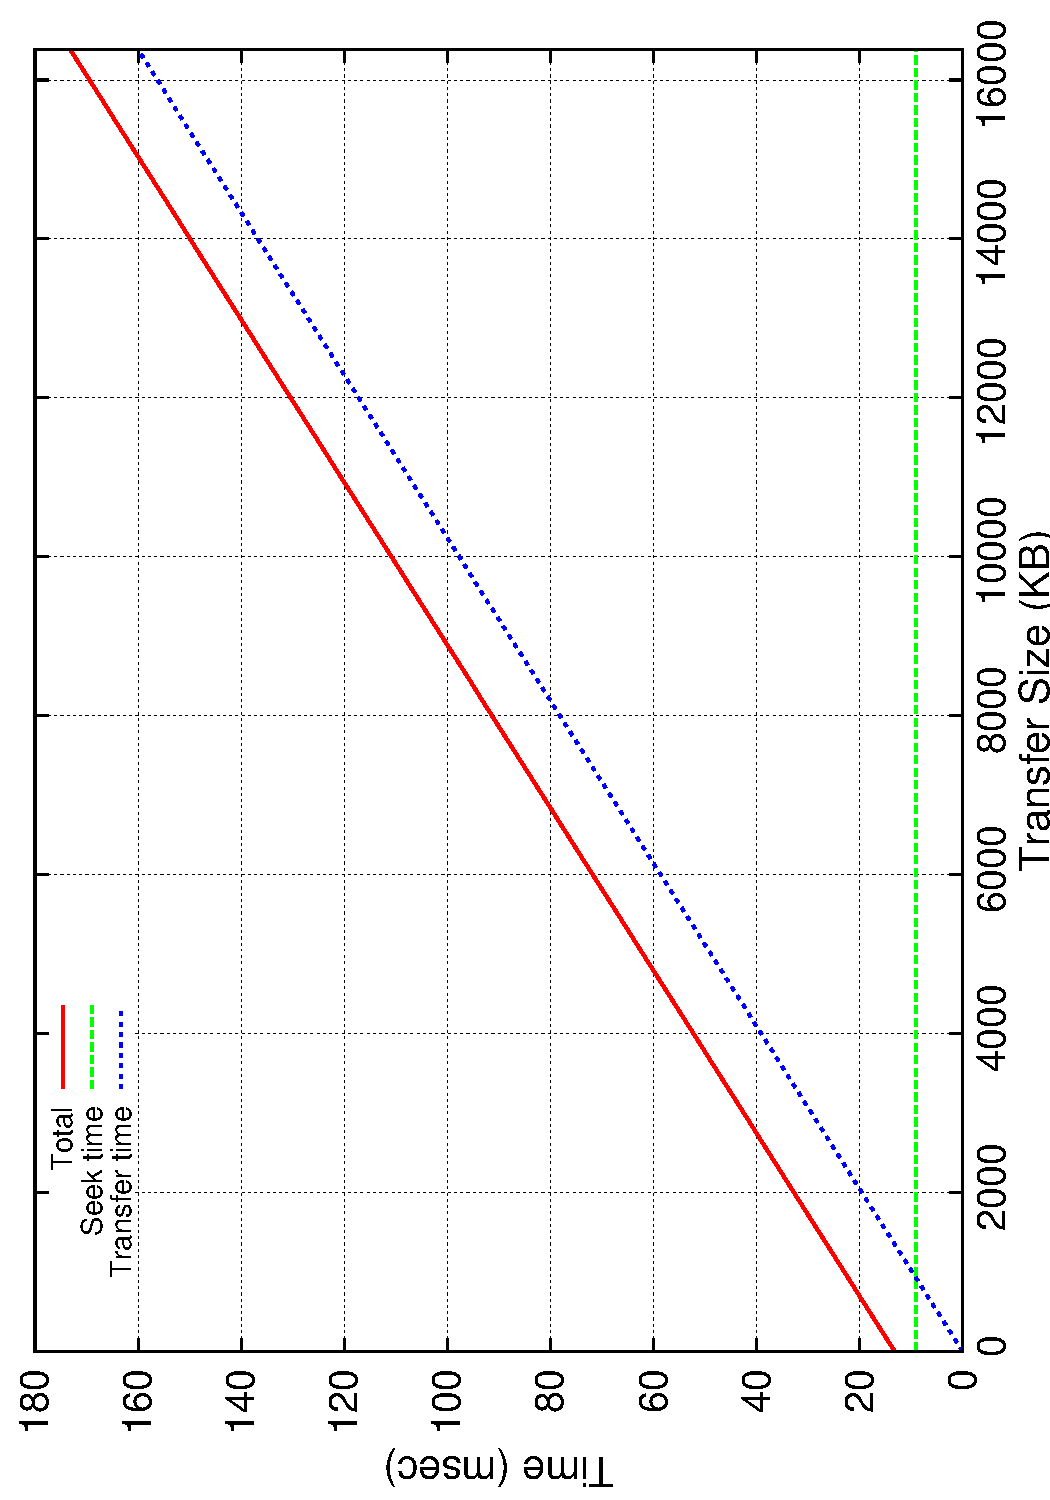
\includegraphics[angle=270,width=\linewidth]{images/io/io-overall}
  \caption{Total I/O time as a function of transfer size.  Transfer rate
  quickly overtakes access time.}
  \label{fig:io-total}
\end{figure}

%%%% It the transfer rate section goes this one should follow
%Since it is very hard to optimize for $T_{rotational}$ we will
%focus on seek time and transfer time optimizations in the following
%sections.

\subsection{Considerations for access time optimizations}

The total time to transfer data of $M$ MB can
be described by the equation:
\begin{align*}
  T_{total} =  \frac{T_{\text{access}}}{1000} +  \frac{M}{R_{\text{trans}}}
\end{align*}
where $R_{trans}$ denotes the transfer rate in MB per second. 
We divide $T_{access}$  by 1000 to express it in seconds as it is
normally given as milliseconds.
Consequently, the access time represents a percentage $P$ of the overall time,
which can be expressed as:
\begin{align*}
P &= 100 \cdot \frac{T_{\text{access}}}{T_{\text{total}} \cdot 1000}
\\&=  \frac{T_{\text{access}}} {\frac{T_{\text{access}}}{100} +  10 \cdot \frac{M}{R_{\text{trans}}}}
\end{align*}
If we now insert the parameters of the above described hypothetical
disk and assume that we are partitioning our data in 10 MB blocks we
arrive at the consclusion that---when we need to do a random seek
operation for every single block of data---the seek time accounts for
only 7\% of the overall time to access the data.

Now, to assess the gain of a specific layout scheme we consider the following 
equation. It measures the performance gain $G$ in percent for a given scheme if that scheme reduces 
random access by a factor of $F$.

\begin{align*}
G  &= 100 \cdot F \cdot \left( \frac{ \frac{T_{\text{access}}}{1000} + \frac{M}{R_{\text{trans}}} }{\frac{M}{R_{\text{trans}}}}- 1\right)
\\ &= 100 \cdot F \cdot \frac{ \left(\frac{ T_{\text{access}} } {1000}\right)}   { \left(\frac{M}{R_{\text{trans}}}\right)}
\\ &=  \frac{F}{M} \cdot \frac{T_{\text{access}} \cdot {R_{\text{trans}}}  }   { 10 }
\end{align*}

Again, assuming the hypothetical drive parameters from above and we get

\begin{align*}
G  &=   \frac{F}{M} \cdot 80
\end{align*}

For a scheme that reduces random access by a factor of 3, only a 2.6\%
improvement in runtime would be achieved for 10 MB blocks, while with the same scheme
the performance would be almost tripled with 900 byte blocks.

From these numbers we conclude that in most environments, in particular
those with structured data---where larger data blocks can be
utilized more easily---a data layout optimization would only improve
a very small fraction of the overall time and is most likely not worth
the implementation and
maintenance effort. For environments that \emph{must} break the data into
tiny chunks a clever layout strategy to improve data access times can in the
best case (in which practically all disk operations involve seeks) double the
data access performance.

%%%% moved to ``The takeway:'' to make it more consistent with the 
%%%% rest of the paper
%Looking at the above results from a different perspective, we can derive the
%rule of thumb that as long as data is broken into pieces larger than 10 MB
%no special care needs to be taken on a consumer HDDs about the data layout.  

It is worth noting that with the advent of solid state drives, in
particular for consumer workstations, this minimal block size required
to utilize unwrought data layout strategies while still obtaining
good performance is bound to shrink even more, as those drives have a
significantly smaller `seek' time with only moderately higher transfer
rates.

Finally, it should once again be stressed that the percentages
given above account for maximum theoretically possible optimization
potentials if all seek operations could be completely avoided and no
other additional overhead would come from the layout.  In reality the
speedup that can be gained from access time optimization will stay
below that value. In particular it is worth noting that accessing data
via optimized layout schemes does not come
for free. Kendall et al.~\cite{Kendall:2009:TDO} demonstrated for
distributed memory systems that a random ordering scheme outperforms
most space filling curve approaches.

The takeway:

\begin{itemize}
  \item If the data is broken into pieces larger than 10 MB, then it
  is not worth worrying about the data layout for even consumer level
  disks.
  \item For kilobyte sized chunks a clever layout strategy can
           significantly cut the data access time on a standard HDD.
\end{itemize}

%% Great idea, no time.
% \subsection{Considerations for transfer time optimization}
% 
% \todo{Should the experiments show that it makes sense to 
% use compressed data then talk about how modern processors
% have so much horsepower that it makes sense to reduce the
% size of the data at the cost of more CPU cycle to prepare it. 
% Give a bunch of numbers/graphs that demonstrate this behavior
% with a number compression algorithms, CPUs, and disks.}

\section{Parallel Filesystems}\label{sec:parallel_fs}

All distributed filesystems have unique characteristics which should
inform the way we access and process data.  In this section we
will highlight some of the common pitfalls that may be found with
applications designed to run in an NFS or Lustre environment.

\subsection{Opening Files}

Opening a file is one example of an operation which performs uniquely
in a distributed environment.  In NFS systems, this is implemented
via the client sending an \verb!ACCESS! or \verb!GETATTR! remote
procedure call.  The operation asks the server if the client is allowed
to access the file, or requests metadata for the file.  The server
responds with a small message containing the resulting permissions.
The situation in Lustre is similar: queries go to a global `metadata
server' (MDS) which determines access information.  In both systems,
\emph{the file is not opened}.  Doing so would consume resources on
the server, particularly due to read-ahead caching, and the request
to actually read or write the file may be significantly delayed in
time---or might never come at all!

%\begin{figure}[Htb]
%  \centering
%  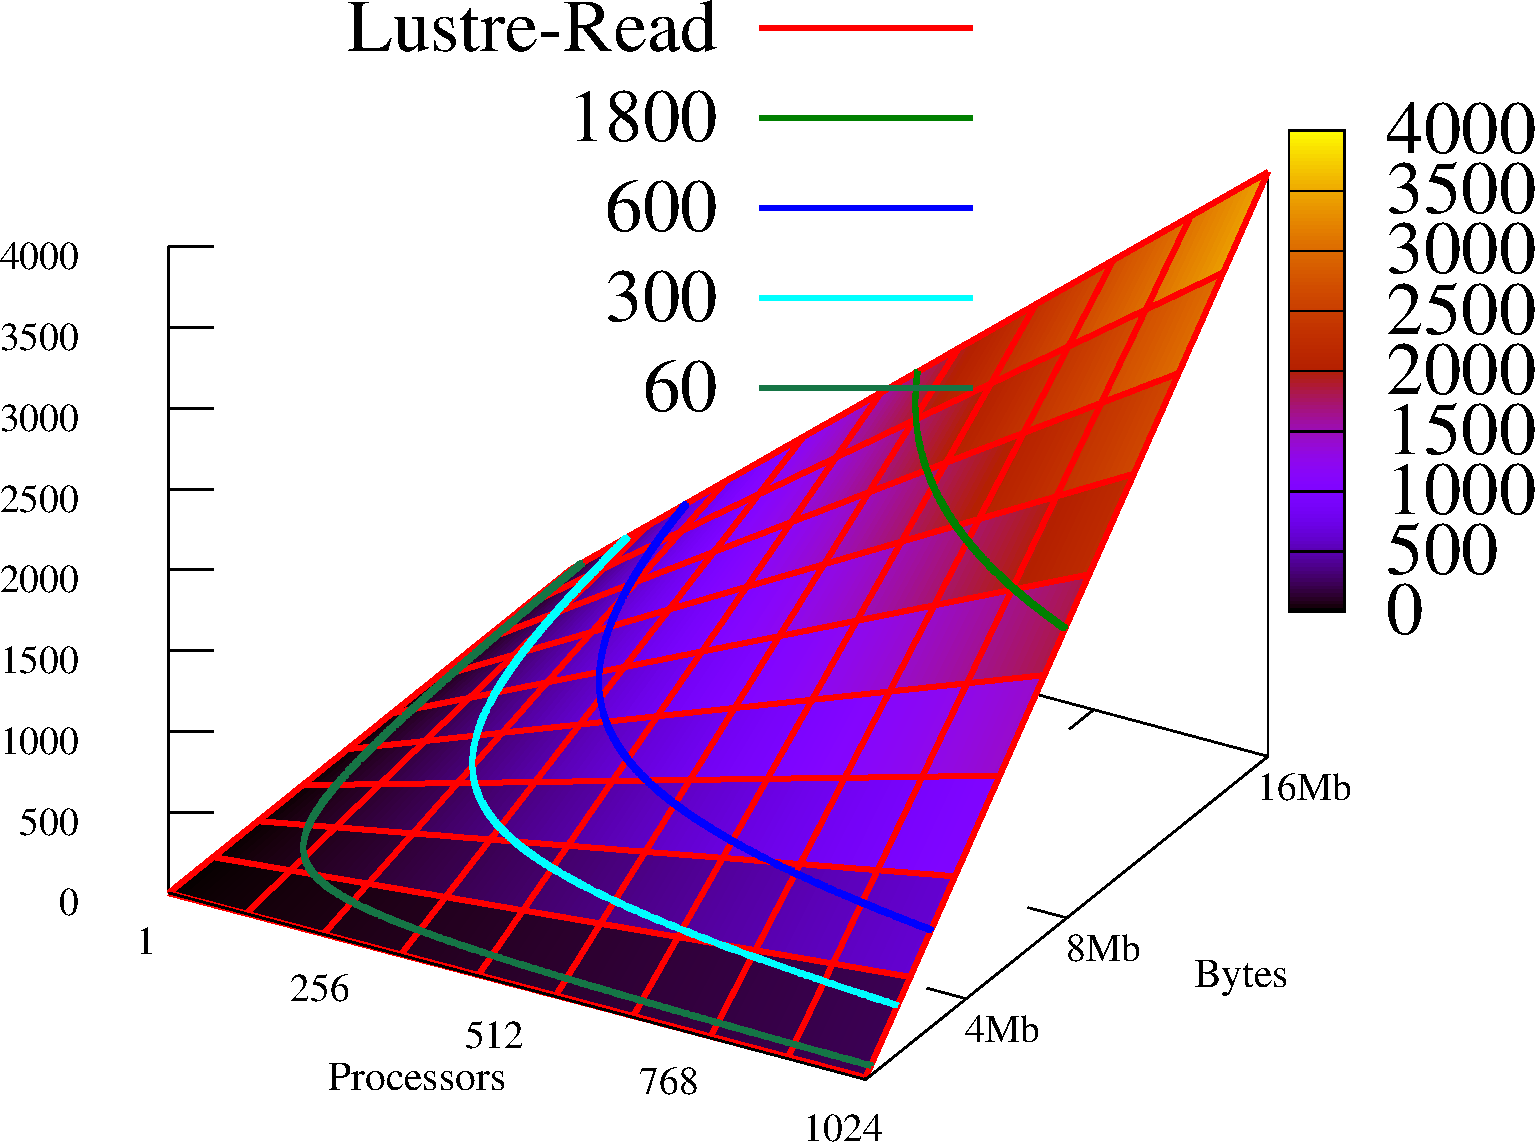
\includegraphics[width=\linewidth]{images/io/lustre-read}
%  \caption{Best case read performance with Lustre. \todo{Fits?}}
%  \label{fig:lustre-read}
%\end{figure}
%
%\todo{Can we fit/justify Figure \ref{fig:lustre-read} in here somehow?  It's
%such a pretty graph ;)}

This has important implications for programs running on such
filesystems.  Any distributed filesystem is going to scale extremely
poorly with a program that opens many files at one time.  Since the
\verb!open! call must correctly report errors, the request and response
must be entirely synchronous.  There is no \verb!openv! system call in
POSIX, analogous to \verb!readv!.  Therefore every open file request
must send a (very small) message to a server, and wait for a (very
small) message to return.  The network capacity for messages at these
sizes is extremely poor.  It is important to note that \emph{Lustre
does not scale any better than NFS} in this use case, as it has the
singular bottleneck of one MDS per filesystem.  Many sites split up
their Lustre offerings into multiple filesystems as a way to mitigate
this problem, but of course these must then be mounted under different
locations in the filesystem hierarchy.

To prevent inducing poor performance in this manner, avoid opening
more than one or two files per process; at large scale,
even that will be a bottleneck.  Furthermore, if at all possible,
avoid synchronization points immediately before opening files: if one
absolutely needs an \verb!MPI_Reduce!, for example, try opening the
file immediately before the reduce instead of immediately after.  This
should prevent a `thundering herd' (to steal a term from the threading
world) of processes which pound on the metadata server at the same
time.  It is interesting to note that the ADIOS middleware library
already attempts to mitigate this effect~\cite{ADIOS:Manual}.

The takeway:

\begin{itemize}
  \item At large scale, eschew large numbers of files.
  \item Stagger synchronization points with \verb!open! calls.
\end{itemize}

\subsection{Closing Files}

Distributed filesystems almost unilaterally implement what is referred
to as `close-to-open cache consistency'.  To increase performance,
writes are cached locally on the client filesystems.  During regular
intervals or in response to certain events, the client cache is flushed
to the server.

This presents difficulties in implementing \verb!write!s.  The problem
is in reporting errors when a write should fail; since the system only
writes to a local cache, the write never reaches its final destination
and thus additional errors could still occur after the user process has
proceeded beyond the write.  It is possible for the write to be sent to
the server machine, enter into the server's cache, and eventually be
denied due to a transient error (e.g. exceeding quota).  Yet the client
system cannot report this error to the running process, because the
process has long since moved on from the failing write call.

Distributed filesystems thus require a client cache to write-through
all changes when the client application closes the file.  Client
operating systems must get a confirmation from the server that all data
has been flushed
\emph{before} it returns from the client processes' \verb!close!
call; this is the last possible operation for the file, and thus the
distributed systems' final opportunity to report errors which may
indicate data loss.

It is therefore highly desirable to delay close operations which occur
after writes.  If a process is writing multiple output files, try to
make it maintain two open files instead of one, and close the file from
the previous iteration while writing in the current iteration.

Sadly many applications, even those designed to run on supercomputers,
do not check the return value of the \verb!close! system call.  There
is no reason to believe that what was written is at all valid, given
such applications.

The takeaway:

\begin{itemize}
  \item \emph{Always} check \verb!close! for errors!
  \item Try to delay \verb!close!s that appear after \verb!write!s.
\end{itemize}

\subsection{Locking}

By `locking' here we are referring to advisory file locking, a la
the \verb!flock! system call; mandatory file locking has its own
set of issues in even a serial environment, and the utility of such
locking in an HPC environment is nebulous.  In our experience, few
if any large scale visualization and analysis applications utilize
file locking.  However, it is worth noting that locking typically
adds an I/O synchronization point, much like \verb!close! would.  For
this reason it is not recommended that an application lock and unlock
files unless there is an interaction with known external software
which dictates it.  If at all possible, a better solution would be
to \verb!close! the files on the writing process, and send a message
to reading processes notifying them that the writer has completed --
before they attempt \verb!open!ing the files at all.

Locking can in theory provide the best mechanism for inter-process
communication in a distributed environment (i.e. to coordinate with in
situ visualization and analysis processes), however it is not in wide
use, perhaps due to the issues mentioned here.  As noted
earlier~\cite{Ching:2007:Locking}, this is still an area of research
in HPC systems and so we recommend the aforementioned explicit
synchronization methods for now.

\section{Parallel Data Access}\label{sec:access}

To identify the ideal method for accessing data in numerous
environments, we wrote test programs using a variety of APIs and
API options, then evaluated their performance.  Yet many scientific
visualization and analysis packages, in addition to large scale
simulation software, utilizes some I/O middleware for data access.
These middleware packages offer complexity reduction, and typically
provide a method for ascribing higher level metadata with data, such as
the dimensionality and mesh information.  After identifying the ideal
low-level methodologies, we sought to quantify the differences between
middleware libraries, and in particular their scalability on distinct
clusters.

To quantify this, we developed the same analysis program using
a variety of backend APIs.  The program is simple: it is a
threshold-based volume segmentation tool.  The software reads in a
large volume and outputs a binary mask volume which indicates the
voxels which fall between the threshold values.  The program is
parallel, and out-of-core: the input volume is intelligently bricked,
and each process is responsible for a set of bricks.  Processes load
up a brick and generate an output brick one at a time.  We chose
out-of-core as opposed to in-core because it models how future (even
current) visualization and analysis software must be written, given the
current trend of increasing processing-power-to-memory ratios.

% .. could add it if we need to fill space.
%\todo{Figure with pseudocode for the program?}

\subsection{Results}

We ran our application on multiple distinct supercomputers.  One
cluster is specifically designed for visualization; another excelled at
analysis; the third is a very large scale general purpose supercomputer
designed for `leadership computing'.  Installation dates were diverse:
one cluster was commissioned in 2008, another went into production
early in 2010, and a third was originally installed in 2005, receiving
its most recent upgrade in 2009.  All of these clusters are using
Lustre for their backend filesystem.  On all systems, we used the
`native' compilers and, where available, system-installed modules for
the libraries we required.

% lens: installed may 2008 (analysis)
% longhorn: production on jan 4th 2010 (visualization)
% jaguar: installed 2005, upgraded late 2009 (general purpose)

For backend I/O we tested multiple configurations: NetCDF, HDF5/NetCDF,
and a custom solution.

The hierarchical data format (HDF) is a data model which has seen
significant uptake in the parallel computing world.  It provides
mechanisms for organizing complex data in an extensible manner.  We did
not look directly at HDF5, but instead considered it in concert with
NetCDF.

\begin{figure}
  \centering
  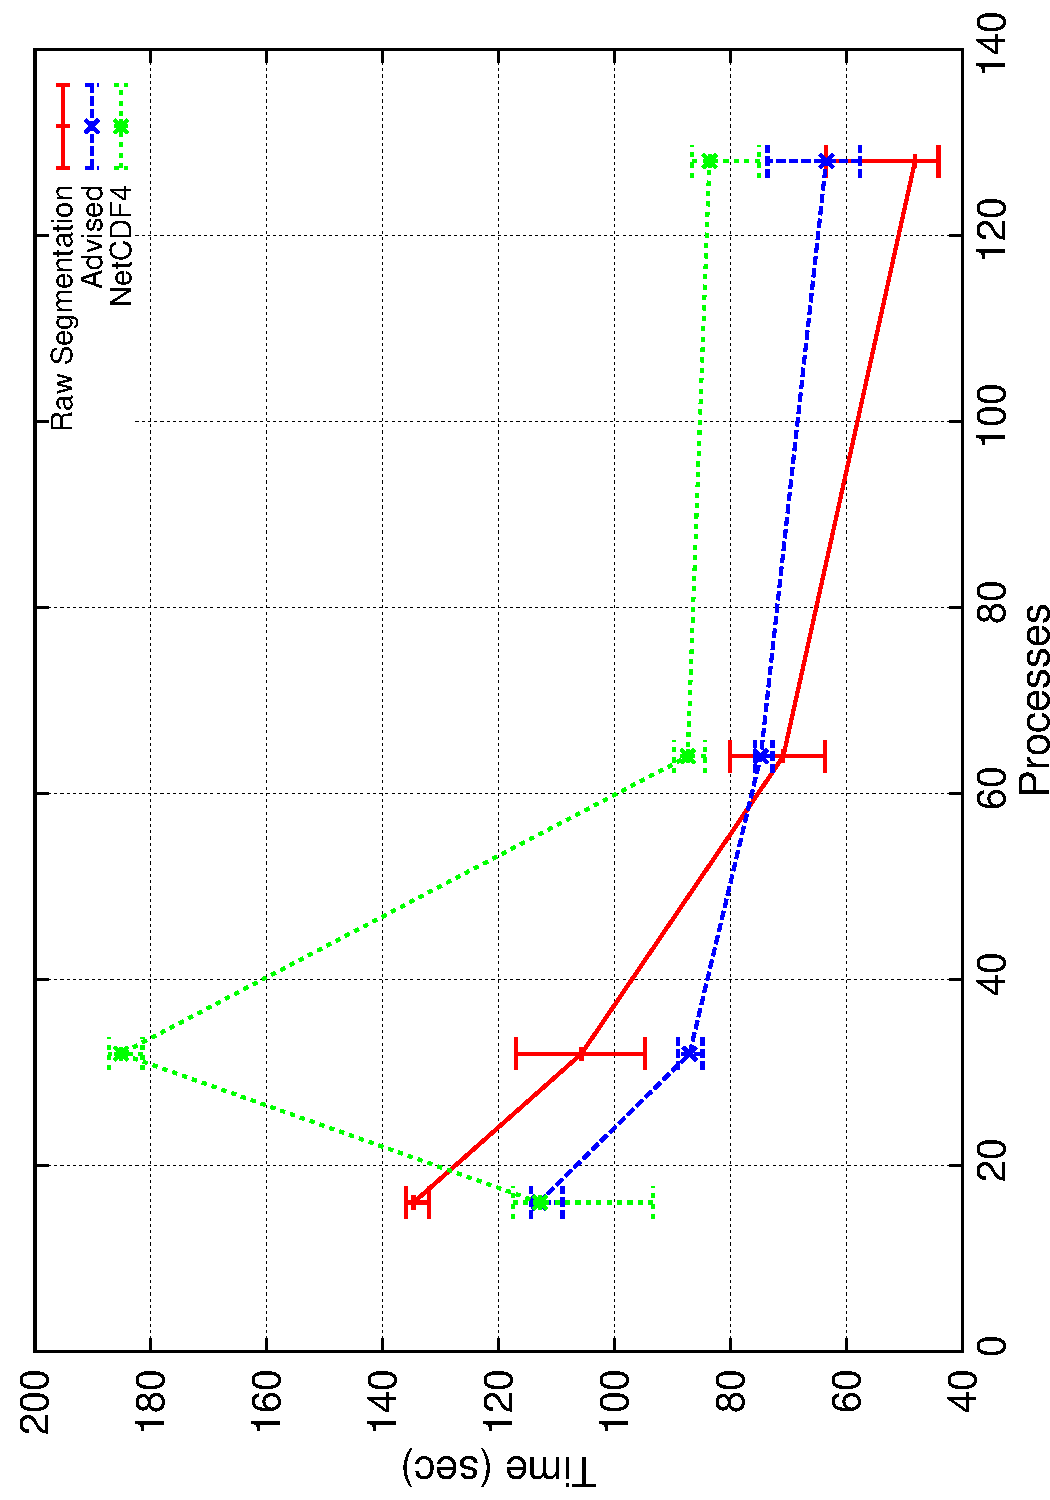
\includegraphics[angle=270,width=\linewidth]{images/io/lens-most}
  \caption{Strong scaling of our example segmentation program running
  on cluster \#1, with a variety of I/O backends.  `NetCDF4' is NetCDF
  with an HDF5 backend.  `Raw' is our hand-generated simple I/O layer,
  and `Advised' a minor modification on it.  Error bars indicate
  maximum and minimum running times per process in the job.}
  \label{fig:lens-most}
\end{figure}

The Network Common Data Form is a library which provides array-oriented
data access.  Like HDF5, NetCDF files endeavor to be partly
self-describing.  With recent releases of the NetCDF library, there
are a multitude of options for backend I/O.  The first is so-called
`classic' NetCDF files.  These files have a limit of 2Gb per variable,
and thus were not considered for this study.  The `64bit offset' format
is an extension of the `classic' format to allow use of 64bit indices,
and thereby to address files of, for all practical purposes, unlimited
size.  The final format is the so-called `NetCDF4' format -- somewhat
confusing because the `64bit offset' format debuted in 3.6.0, right
before the 4.0 release, yet is a distinct backend -- which uses HDF5 as
its backend.  To disambiguate, we refer to the `64bit offset' format as
``NetCDF-64'' and the HDF5-backed format as ```NetCDF4'' in this work.

We also developed a custom I/O layer based on our experiences on a
variety of machines, including workstations.  The approach is very
simple: each process memory-maps a chunk of the large input data file,
as well as the relevant portion of the output mask file.  Data are
processed out of the memory-map as is, without intermediate buffers.
The source for this version is thus simpler than any other version of
the program, containing no memory management code for data buffers.  As
such, this version required the least memory by a wide margin: the API
dictated an approach which was naturally out-of-core.

The results on the first cluster can be seen in Figure
\ref{fig:lens-most}.  `NetCDF4' is NetCDF backed with an HDF5 file.
`Raw segmentation' uses our custom I/O layer based on \texttt{mmap}.
`Advised' is the `Raw' line, with the addition of just a single line of
code, placed before we process a block of data:
\begin{verbatim}
  posix_fadvise(fd,
    index * sizeof(float),
    buffer_size,
    POSIX_FADV_WILLNEED
  );
\end{verbatim} That is, we are informing the operating system that
we will need block $X+1$ in the near future, just before we begin
processing block $X$.  We had found that including this optimization
increases our performance 3 to 4x on desktop systems.  Results on the
supercomputer do show an initial increase in performance, but the
effect was unfortunately subdued at higher concurrency.  We do not
include results for the NetCDF-64 run in this figure, as it did not fit
in the same scale as the pictured backends.

Results for this machine were somewhat difficult to report, because
they varied so widely.  We ran the scaling study for one particular
format straight through, with no delays between runs, multiple
times.  In each instance the NetCDF4 result included a spike in the
running time.  For our raw segmentation, we would see results offset
by 20 seconds or so, and the width of the error bars would change
arbitrarily.  The readahead version of the program experienced less
variability, but we were unable to conclude whether this was a property
of the program or simply luck.  The data presented in figures
represents the \emph{set} of runs which performed best overall, for
that I/O backend.

\begin{figure}
  \centering
  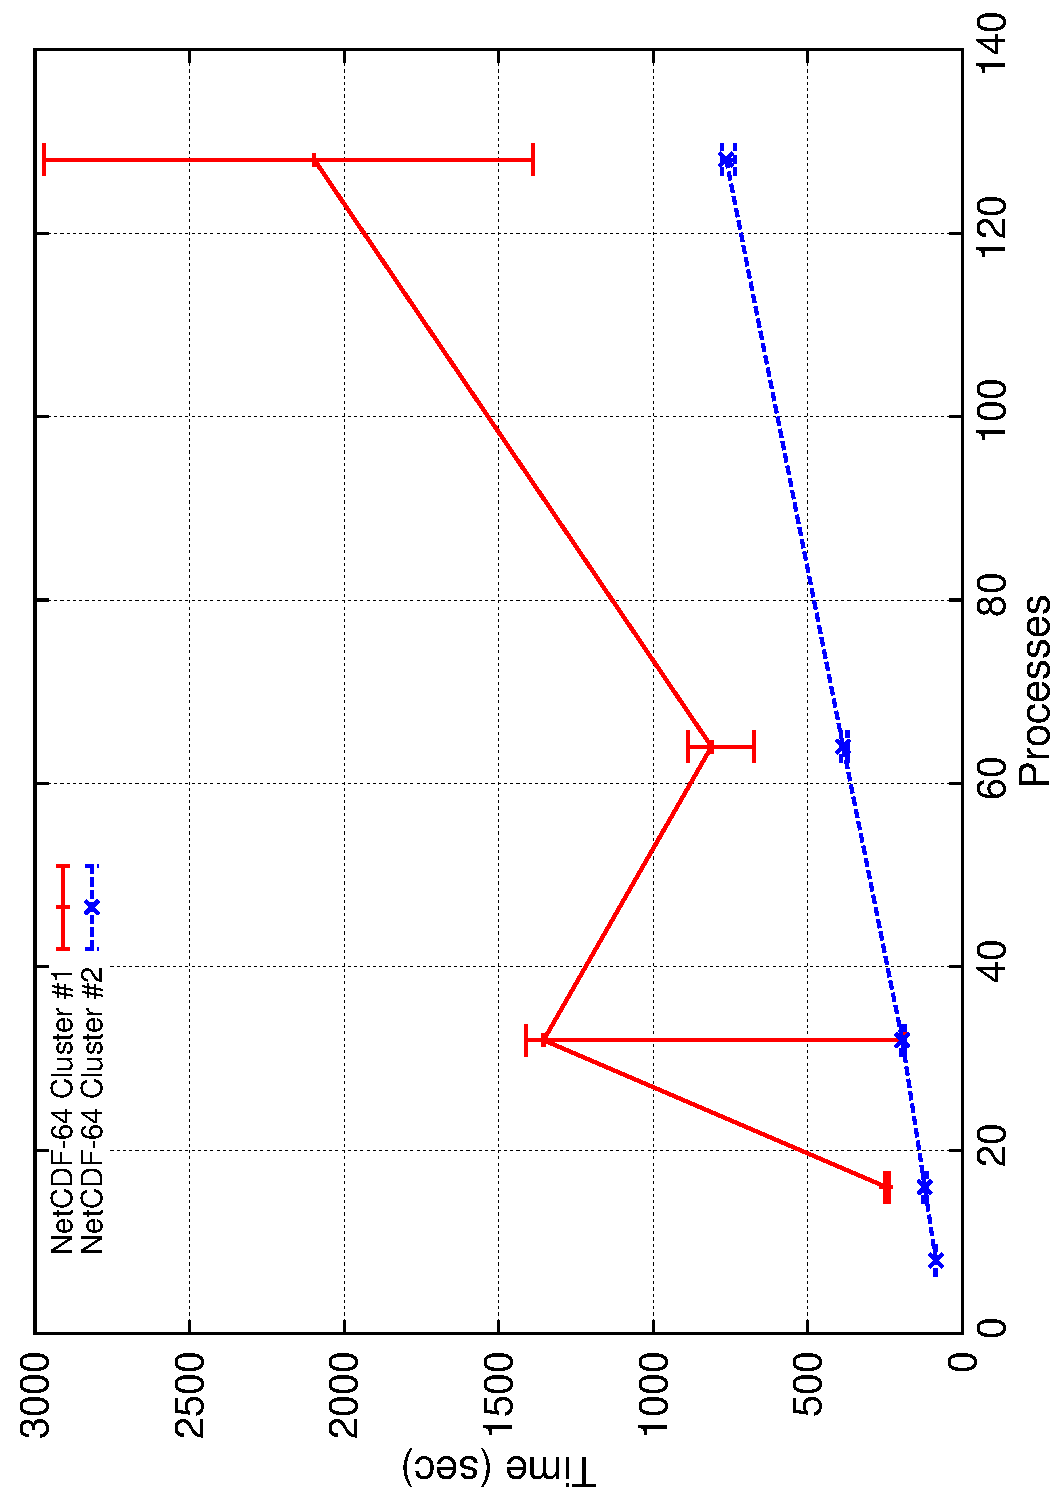
\includegraphics[angle=270,width=\linewidth]{images/io/n64}
  \caption{Strong scaling using the NetCDF `64bit offset' file format
  on multiple clusters.  Higher levels of concurrency led to decreased
  overall performance when using this format.  Of note is the high
  variability from cluster \#1, characteristic of that machine's I/O
  subsystem.}
  \label{fig:n64}
\end{figure}

The NetCDF-64 results could not be plotted with the other results, due
to the large difference in scale.  Results using this format on
multiple clusters is provided in Figure \ref{fig:n64}.  Performance
actually decreased with this backend.  For this reason, we highly
recommend forcing the HDF backend (using the \texttt{NC\_NETCDF4} flag)
when writing applications which make use of the NetCDF API.

\begin{figure}
  \centering
  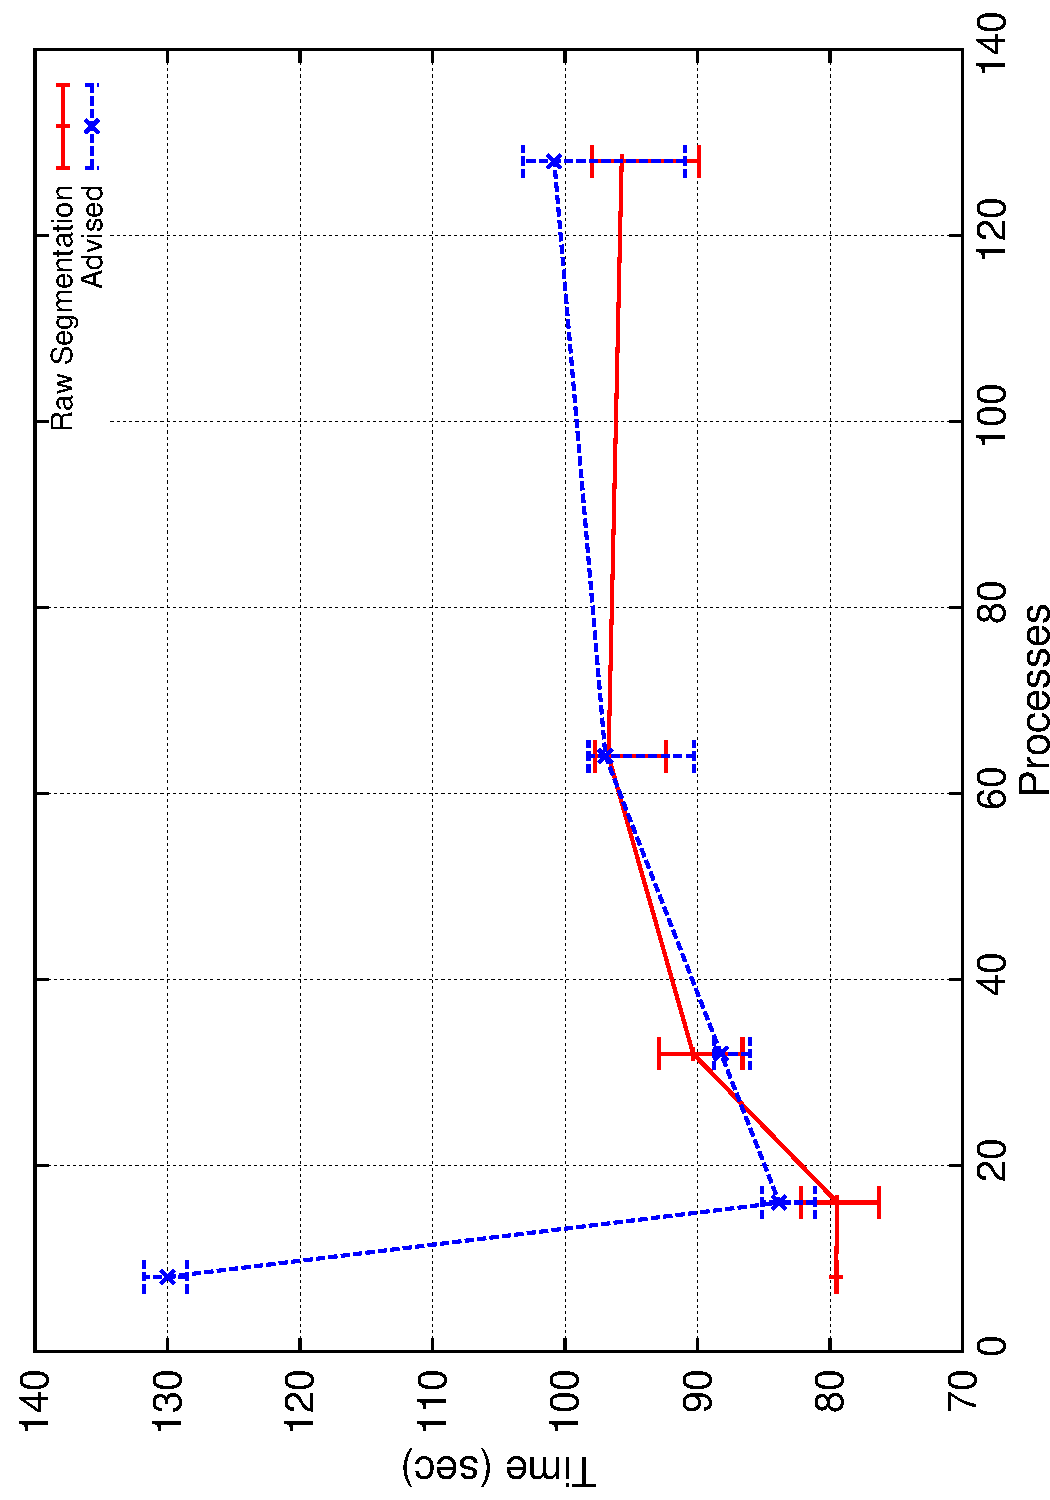
\includegraphics[angle=270,width=\linewidth]{images/io/lh-most}
  \caption{Raw segmentation strong scaling with and without explicit
  caching, on the second cluster.  Explicit single-block readahead
  makes little difference, especially at higher concurrency levels.}
  \label{fig:lh-most}
\end{figure}

Results from running on the second cluster are given in Figure
\ref{fig:lh-most}.  The HDF-backed NetCDF version could not be run on
this cluster due to a software incompatibility.

\begin{figure}
  \centering
  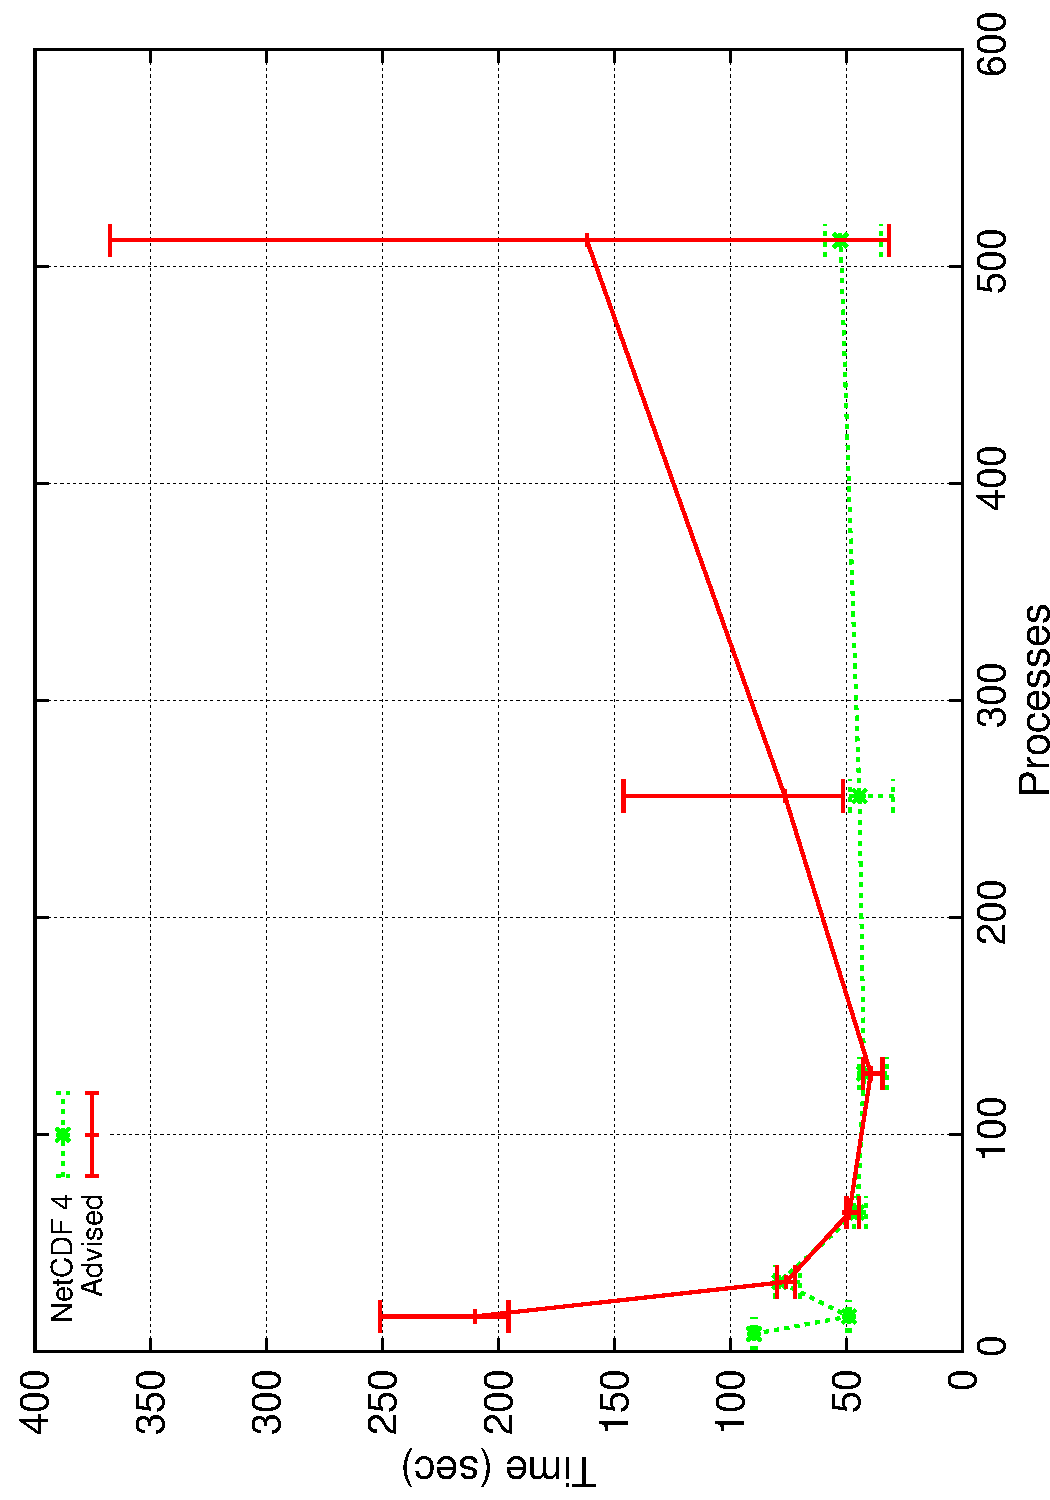
\includegraphics[angle=270,width=\linewidth]{images/io/jaguar-most}
  \caption{HDF-backed NetCDF and raw advised I/O method scaling on the
  third cluster.  Performance is largely the same at first, hinting
  that explicit readahead is likely too limited to be effective.  At
  higher levels of concurrency, our writes get very small, and the HDF
  backend is able to deal with the case much more effectively.}
  \label{fig:jaguar-most}
\end{figure}

Results from the third cluster are given in Figure
\ref{fig:jaguar-most}.  This machine is one of the largest scale
supercomputers we have access to, and so we performed runs at larger
levels of concurrency, although we did not utilize the entire cluster.
We only performed the `advised' version of our raw algorithm for this
cluster, as the simpler version gave essentially the same performance,
and compute time was harder to obtain for this machine.

%\subsection{ADIOS}
%
%ADIOS is unique in that it is not a file format alone, but rather a
%middleware suite that interfaces to a variety of backend methods for
%reading and writing data.  These methods include HDF5, NetCDF4 and
%ADIOS-only backends such as raw POSIX I/O and MPI-IO.  One of the
%promising features of this approach is that such a system could have
%rapid uptake of the results presented in work such as this.
%
%Unfortunately the current release at the time of publication (ADIOS
%1.2.1) does not yet support out-of-core data access.  For large-scale
%visualization applications, which commonly run on just a subset of the
%nodes utilized to produce simulation data in the first place, this is
%an essential feature.  We hope to include ADIOS results in a future
%study.

% Would be nice.. no time now.
% \todo{They actually have pretty good documentation on how to add a new
% transport method... though not a new API.  Still it's probably simple.
% Maybe we could add an out-of-core API to ADIOS and evaluate it here
% quickly enough?}

%\subsection{Custom Low-Level Data Access}
%
%This is a method we developed based on a series of experiments with
%different I/O methods on multiple machines.  The approach is rather
%simple: each process memory-maps a chunk of the large input data file,
%as well as the relevant portion of the output mask file.  Data are
%processed from the memory-map as-is.  The source is very simple, and
%contains now allocations other than those performed internally (for
%example, to initialize MPI).  As such, this version of the program
%required the least memory by a wide margin; the natural method of
%writing it was out-of-core.

% \begin{figure}
%  \centering
%  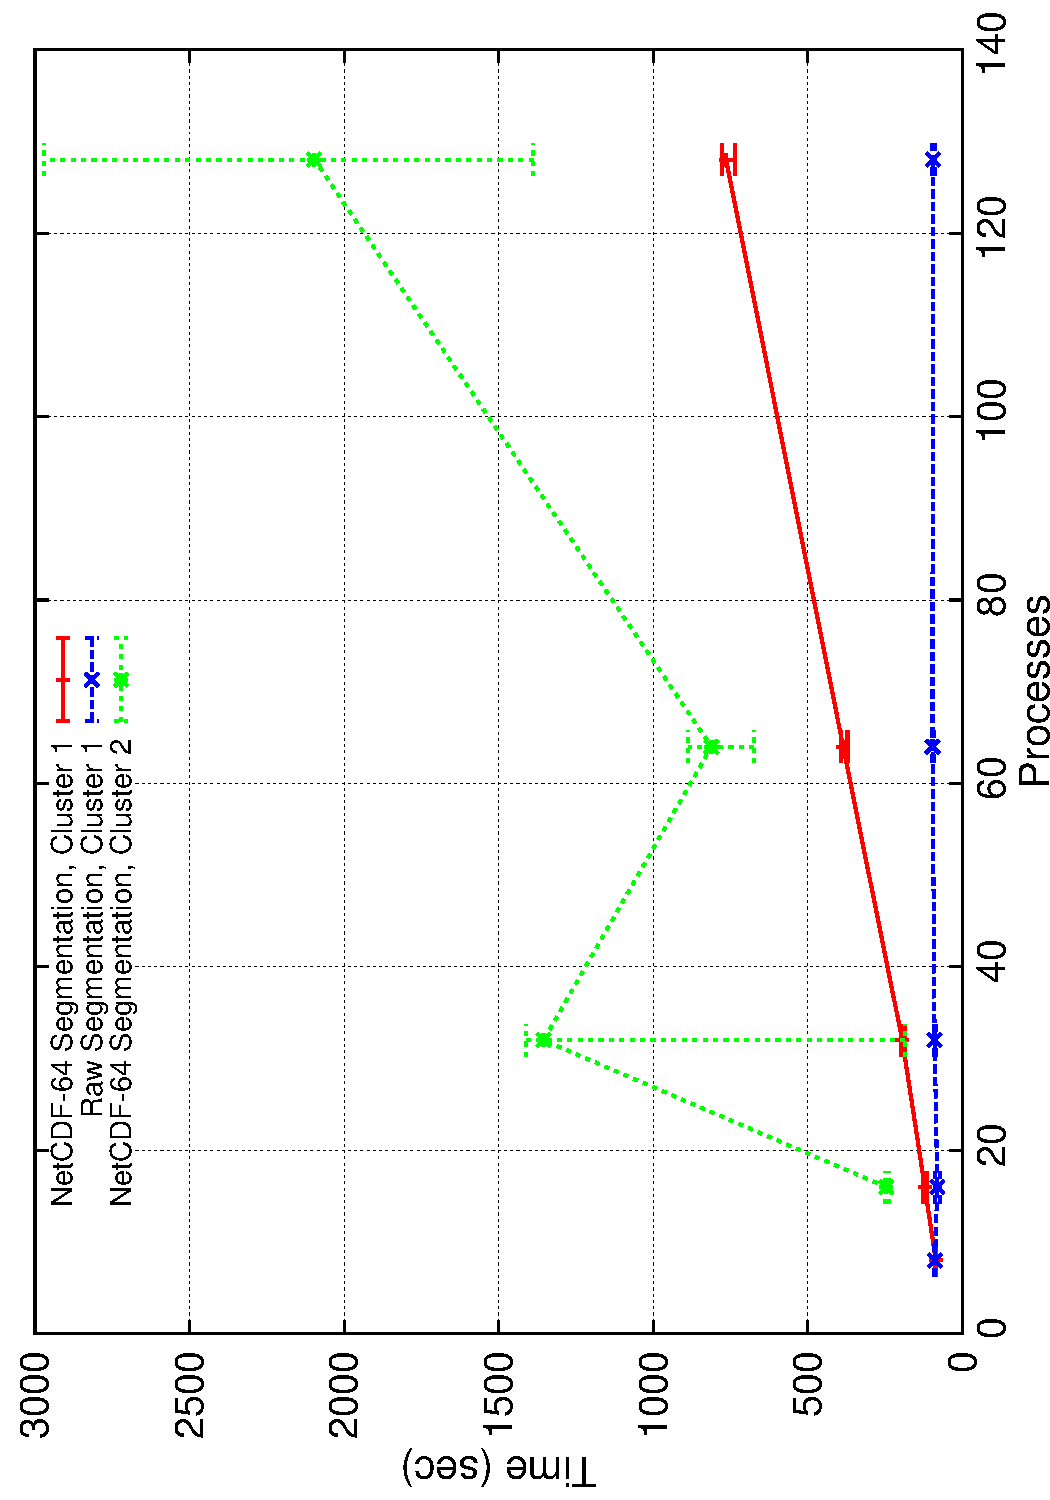
\includegraphics[angle=270,width=\linewidth]{images/io/lh-all}
%  \caption{
%  Strong scalability for a simple segmentation problem using NetCDF
%  `64bit offset' files and a custom I/O layer, on multiple clusters.
%  Error bars indicate minimum and maximum running times observed, per
%  process in the job.
%  \todo{split things into two figures: one figure for Lens, one for Longhorn,
%  and another for Jaguar if I can fit runs in...}
%  }
%  \label{fig:lh-performance}
%\end{figure}

% Figure \ref{fig:lh-performance} shows the scalability of this program
% (`Raw Segmentation') alongside the results of the NetCDF4-backed files,
% run on the same cluster\todo{err, multiple clusters now, but will
% be split up later...}.  At scale, the performance appears to be
% flat.  However, we note that a closer look at the performance data
% indicates that performance increases up to 16 processors, and then
% begins to worsen.  This is due to our chosen problem; the thresholding
% segmentation is incredibly simple, and after 16 tasks we don't gain
% much of a benefit from more processors, as there simply is not enough
% work to go around.

% \todo{Do some runs with a 1 terabyte file or similar (current file
% is 32gb, $2048^3$). Use this in the text: ``While we don't show the
% results, we ran the raw tests with a larger file, and confirmed that
% more processors brings the runtime down out to a larger number of
% processors, demonstrating that we just do not have enough work in our
% algorithm to scale this approach appropriately.  More complicated
% applications would see a greater benefit from this method.'' blah
% blah blah}.


% This is still true, but the raw benchmark kicks so much ass that I
% don't think we need to go back and redo the NetCDF benchmarks &&
% ensure we're comparing apples-to-apples.
%\note{The raw I/O benchmark includes the `close' calls, but the
%(currently-running) NetCDF benchmarks you have going do not.  Probably
%want to go back and redo the NetCDF benchmarks to time that.}

\section{A Parallel File API}\label{sec:design}

In the work presented for this paper, as well as our previous
experience writing visualization and analysis programs targeting
supercomputers, we have noticed that the available I/O models presented
by the standard POSIX API is insufficient from both the producer and
consumer vantage points.  Implementers are not given enough information
about access patterns that applications are utilizing, which prevents
them from optimizing the I/O for common tasks.  Library and application
developers, on the other hand, have no mechanism for communicating such
information.  The result is sub-par performance, with both parties
feeling like there is little that can be done.

For this reason, we present an API which:

\begin{itemize}
  \item models the way visualization and analysis application
  programmers think about their data,
  \item simplifies data access, and
  \item enables implementers to design effective filesystems.
\end{itemize}

A summary of the methods which the API provides is given in Table
\ref{tbl:api}.  Our primary goal with such an API is to encourage
application developers to structure their code in such a way that it
models a similar API, as it provides more information to lower levels.
At the same time, we hope middleware libraries and even kernel code
begin to offer APIs which allow application developers to provide this
kind of information.  In the end, there should be much more data about
the patterns and intent of data access that the application provides to
the levels which can make use of it.

\colorbox{lightgray}{\texttt{open\_range}} and
\colorbox{lightgray}{\texttt{close\_range}}; \verb!open! and \verb!close!
calls which work with byte ranges.
One of the issues that plagues I/O concurrency
at large scales is the inability to indicate which portion of data
a process intends to
access: each process only needs some subset of the overall data, but
cannot communicate this a priori to middleware or the runtime system.
To perform effectively in the majority of cases, caching, large stripe
sizes, and readahead must be employed by the I/O system.  However these
techniques create false sharing when byte ranges overlap.

A popular method to combat this problem is to create a single file per
process.  Since only one process accesses the file, it is clear to
the I/O subsystem that concurrent access is impossible.  While this
is effective at the small scale, at the highest levels of concurrency
the method becomes untenable due to overwhelming amounts of metadata:
listing all files in a directory would require making a hundred
thousand requests to a server.  Even if this were technically feasible,
it presents significant data management difficulties; it would be much
easier on users if we could contain results into a singular file.

Many analysis applications would be able to calculate the byte offset
they will need on a given process given just the total number of
processes and the dimensions of the dataset (or number of points in
a point mesh).  Visualization software may need to produce a spatial
hierarchy of the data, but again this can be done with relatively
little metadata.  By providing this information to the underlying
I/O subsystem up front, application developers can cleanly solve one
of the more difficult problems in defining distributed file systems:
distributed lock management.

It should be an error to specify a byte range beyond the file length
when opening a file for read-only access.  When used for write access,
this would be a viable method for extending the file's length.  All
offsets from a file opened in this manner are relative to the start of
the byte range.  Attempting to read beyond the end of the byte range
results in end-of-file.

If the API is made to work with existing file descriptors, the standard
\verb!close! call is the only API needed.  If this API returns a more
opaque type, an API-specific \verb!close! method will be required.

% \colorbox{lightgray}{\texttt{readdirv}}; a \verb!readdir! that accepts
% some type of globbing mechanism and communicates the result to all
% processes in a group.  Consider a visualization application asked to
% process a simulation's output.  The simulation generally created $N$
% files with a common prefix or suffix.  The visualization application
% must identify what that $N$ was and distribute those files among the
% $M$ processes it is presently running on.  The only ways to do this are
% to: 1) have each application \verb!readdir! and identify the files,
% or 2) \verb!readdir! on the root and broadcast the result.  (2) is
% superior, but it would be better if the machine that did the metadata
% lookup knew it had to broadcast the result.

\begin{table*}
  \centering
  \begin{tabular}{|c|l|}\hline
    \textbf{System call} & \textbf{Description}\\\hline
    \textit{open\_range} & open with an explicit range of accessible bytes.\\
    \textit{close\_range} & clean up resources associated with a
      buffer \\
    \textit{readanyv} & accept a set of blocks and returns when any one
      full block is available\\
    \textit{finished} & asynchronous flush; return immediately, but mark
      buffers as unused.\\\hline
  \end{tabular}
  \caption{Summary of proposed new APIs.}
  \label{tbl:api}
\end{table*}

\colorbox{lightgray}{\texttt{readanyv}}; a read that accepts a number
of blocks and returns one of them.  Many applications can identify
what data it will need using a small amount of metadata.  For the
segmentation application used in this work, for example, we could
compute that easily based only on the total amount of data and the
number of processes in the analysis job.  A volume renderer could
read just the world extents of each block and use that for a spatial
subdivision.  In short, it is common for an application to be able to
make progress given some small subset of its input, as long as each
subset is `complete' in some sense.  This interface allows an API
implementer to do \emph{intelligent} read-ahead; as demonstrated in our
test program, this can provide compelling performance advantages.

The API should return pointers; it should not accept previously
allocated buffers.  The gives the implementer freedom to manage
allocations, enabling flexibility in choices of underlying APIs.  For
example, memory-mapped files generally require page-aligned memory,
which is not provided by \verb!malloc! or \verb!new!, and is more
difficult to use at fixed addresses, as opposed to letting the kernel
choose the mapping.

\colorbox{lightgray}{\texttt{finished}}; an asynchronous flush
operation.  This indicates that the given file (or byte range within
the file, given \texttt{open\_range}) will no longer be used.  The
method returns prior to performing any I/O operations.  It is an
error to read from or write to the given file after performing
this operation.  It is an error to open the given file within the
same process without an intermediate \verb!close! operation.  An
implementation may detect these errors.  It is unspecified whether any
other process sees any modifications to the open file before a future
\verb!close! operation completes.

The intent is to allow a system to better manage its cache and write
throughput.  Should the system experience memory pressure, these cache
blocks are the best candidates to consider for flushing.  If the
network or host resources are currently busy, the system might delay
making the write request until a better time.  This would also allow
an implementation to avoid a `thundering herd' of disk write requests:
mitigated in a system such as Lustre, but a difficult problem in an
NFS-like environment.

It is important to note that, while this system interface was
explicitly developed to deal with the problems of distributed systems,
most calls could provide benefits for applications targeted to typical
workstations.  The issues are largely the same, though the stakes are
higher in a distributed system.  Furthermore, such a system would not
obviate the need for current infrastructure; not all file access can
be made to conform to this model, but the intent is that large scale
applications would be able to effectively utilize these APIs for their
primary I/O needs.

\section{Conclusions}\label{sec:conclusions}

We have presented performance characteristics of modern disks.
Utilizing that information, we evaluated a variety of APIs for
file access with large scale data by implementing the same program
using multiple backends.  Where APIs had options which may effect
performance, we experimented with those options to identify which set
gave the best parallel performance on our chosen problem.  We evaluated
this program on multiple clusters, attempting to identify generalized
practices which application developers could follow to obtain superior
performance in the common case: where they have no control over where
their users will run the released code.

Variability in I/O performance, such as that depicted in Figure
\ref{fig:n64}, was considerably higher than we expected it to be.  In
some cases we observed a job taking twice as long to execute than it
did at another point in time.  This presents a difficult challenge
for interactive visualization and analysis applications, which should
provide the illusion of interactive response yet are highly susceptible
to such latency.  The results encourage the use of progressive or
multiresolution renderers, which can be used to provide real-time
responses in the plausible event that the supercomputer cannot respond
quickly enough.

While the best performance was generally obtained by using operating
system APIs directly, we do not advocate developers use these directly
at this time.  Higher level libraries such as NetCDF, HDF5, and ADIOS
provide mechanisms for self-describing metadata and data attributes,
and can achieve similar performance with the proper configuration,
not to mention providing portability across a wider set of systems.
Instead of having every application developer familiarize themselves
with these to-the-metal APIs, our community should instead work towards
the goal of incorporating these ideas into higher level libraries.
However, some API changes, preferably to accomodate a model more like
the one
presented in Section \ref{sec:design}, could go a long way towards
getting users to write code that can be scaled much more easily.

For application developers, we present the following maxims for
obtaining the best I/O performance possible:

\begin{itemize}
  \item Stagger operations that read or write file metadata.
  \item Read or write in large chunks: 10 megabytes or more.
  \begin{itemize}
    \item This frees the developer from the requirement of
    identifying and implementing intelligent data layout schemes.
  \end{itemize}
  \item Use memory-mapped files whenever possible.
  \item If you can do more, unrelated work before \verb!close!-ing some
  file resource, do so.
  \item \emph{Always} check and report errors during \verb!close!.
\end{itemize}

\subsection{Limitations}\label{sec:issues}

Any study is subject to the limitations of that which can be tested, as
well as the time available to perform tests \textit{ad nauseum}.  This
study is no different, and suffers from at least the following barriers
and limitations on its conclusions.

The most serious is our chosen test application.  We have chosen to
implement a program that essentially maintains two small buffers
at any one time: a brick of the input file and an output brick.
In a real-world application, it would desirable to load as much
data as would fit in the current memory.  Furthermore, many current
applications are not intelligent enough to implement either method:
they employ strictly in-core algorithms.  Due to the memory struggle
between application heap allocations and the operating system's
filesystem caching, in-core applications clearly perform worse when the
heap memory required grows close to the available memory on a node.
%While out-of-core algorithms generally incur some amount of extra
%overhead, this is likely to be negligible.\cite{Fogal:2010:LargeData}
Finally, our application performs very little work on each input voxel;
this was done to emphasize I/O time, but is uncharacteristic of any
useful analysis program.
Therefore it is likely that the application presented here performs
better than real-world visualization and analysis applications.

A second issue, particularly with respect to the proposed API, is
the lack of thorough evaluation.  No applications have been written
to such an API.  We have implemented the API in user-space, but no
middleware or applications have as-yet been adapted to utilize the
model it presents.  Despite these shortcomings, we feel the approach is
well-informed based on our experiences here and in prior literature.

\section{Future Work}

The ADIOS library is unique in that it is not a file format alone,
but rather a middleware suite that interfaces to a variety of backend
methods for reading and writing data.  These methods include HDF5,
NetCDF4 and ADIOS-only backends such as raw POSIX I/O and MPI-IO.
Unfortunately the current release at the time of publication (ADIOS
1.2.1) does not yet support out-of-core data access.  For large scale
visualization and analysis applications, which commonly run on just a
subset of the nodes utilized to produce simulation data in the first
place, we judged this to be an essential feature.  We contacted the
development team and they agreed to look into out-of-core APIs for a
future release; we therefore hope to include ADIOS results in a future
study.

We would like to extend the methodologies used in this work to a larger
set of parallel algorithms.  In particular, algorithms that must
do considerably more per-voxel computation, and those that require
information from neighboring voxels.

% \subsection{Lustre Overview}
%
% Lustre (an almagmation of ``Linux'' and ``cluster'')
% is a distributed file system which is popular in mid-
% to high-end supercomputing facilities. The major claim
% is that Lustre is \emph{scalable}: administrators can
% add disks and new machines to a supercomputer without
% effecting the overall storage performance.
%
% Lustre filesystems are composed of: a single
% \textit{metadata~server} (MDS), many
% \textit{object~storage~targets} (OSTs), and any
% number of \textit{clients}. The filesystem presented
% to the user has standard POSIX access semantics,
% including advanced features such as locking. New
% machines with attached disks (OSTs) register with
% the MDS, and the MDS handles all indexing of data.
% In classic UNIX filesystem terminology, the MDS is
% essentially a collection of inodes and the OSTs store
% the actual file data.
%
% Knowledge of the filesystem's structure is useful in
% designing large-scale visualization applications. For
% example, consider what happens on an `open' of an
% existing file, depicted in Figure
% \ref{fig:lustre-open}.
%
% \begin{itemize}
%
%   \item The client contacts the MDS, sending a
%   filename and access information (read-only,
%   read-write, etc.).
%
%   \item The MDS responds with the basic inode
%   information, as well as a list of OST-to-indices
%   mappings for file locations (e.g. ``bytes 0-512 is
%   on OST hostA at index 6; bytes 512-1024 are on hostA
%   at index 7'').
%
%   \item In almost all cases, the client now contacts
%   the first (or first few) OSTs, trying to fill up a
%   readahead buffer.
%
%   \item \todo{replace this with a figure}
%   \label{fig:lustre-open}
%
% \end{itemize}
%
% Consider what happens when all processes in an MPI
% job open the same file: we get \verb!MPI_Comm_size!
% processors that all send a small message to the MDS,
% which must do a disk seek and read a few blocks
% before sending the data back. Then each of those
% \verb!MPI_Comm_size! contacts the OST with byte 0
% and asks for `cache size' bytes. In all likelihood,
% the MDS can get by with a single seek here, and it's
% transferring a small amount of data, so disk I/O time
% is negligible. However a large number of processes
% all requesting a network buffer takes its toll on an
% MDS. For example, by default the maximum number of
% connections a Linux kernel will have open at any one
% time is 128. If an MPI job tries to open a file on all
% processors, then a hundred thousand processes compete
% for 128 slots.
% \note{open-ro.c tests this case}
%
% The `cost' in the above situation is the summation
% of: N round-trips to the MDS, the time for the MDS to
% read the metadata, N small sends to request data from
% the OST[s], the time to read the data from the OSTs,
% and N times the transfer cost of the given data. More
% succinctly:
%
% % This logic needs to be fixed to account for striping.
%
% \begin{eqnarray*}
%   T & = & N \times T_{send->MDS} + \\
%     &&    1 \times T_{read,MDS} + \\
%     &&    N \times T_{send, metadata} + \\
%     &&    N \times T_{send->OST, request} + \\
%     &&    N \times T_{read, OST} + \\
%     &&    N \times T_{send, data}
% \end{eqnarray*}
%
% Since we consider metadata to be `small', we ignore
% transfer time when the MDS
% reads metadata. Thus $T_{read,MDS} = T_{seek}$, the
% time to seek to the appropriate metadata. We model
% network transfers as taking time $M + nB$, where $M$
% is a constant message setup cost and $B$ is a per-byte
% cost, and we use similar simplifications here,
% discounting per-byte overhead for metadata on the
% basis that $nb << M$. Using those transformations,
% our costs become clearer:
% \begin{eqnarray*}
%   T &=& {} + N \times M  \\
%     &&  {} + T_{seek, MDS} \\
%     &&  {} + N \times M \\
%     &&  {} + N \times M \\
%     &&  {} + N \times (T_{seek} + T_{rotational} + T_{transfer}) \\
%     &&  {} + N \times (M + nB)
% \end{eqnarray*}
%
% We consider network performance numbers as given in a
% now-dated
% paper\cite{Rodrigues:FastSockets:1997}\todo{need to
% find a newer paper that has a table like the one
% found in that one...}; modern networks will certainly
% perform better. Regardless, per-message and per-byte
% overhead is measured in tenths of microseconds; a
% message costs about a third of a microsecond, and a
% byte costs approximately 0.2 microseconds. Therefore
% at just over 4k bytes the per-byte overhead adds up to
% about a millisecond; we can send 37,000 bytes in the
% time it takes to seek on an average disk.  This gives us a function for the
% time taken
% \begin{eqnarray*}
%   T(N, b) &=& {} + 3(N \times 0.3 \mu{}s) \\
%           &&  {} + 9 ms \\
%           &&  {} + N \times (9ms + 4.2ms + b/102400) \\
%           &&  {} + N \times (0.3 \mu{}s + 0.2 b \times 1024)
% \end{eqnarray*}
%
% where $N$ is of course of the number of processes
% in the system and $b$ is the number of bytes to
% read, in kilobytes. The function makes the same disk
% assumptions that we did earlier.
%
% \begin{figure}[Htb]
%   \centering
%   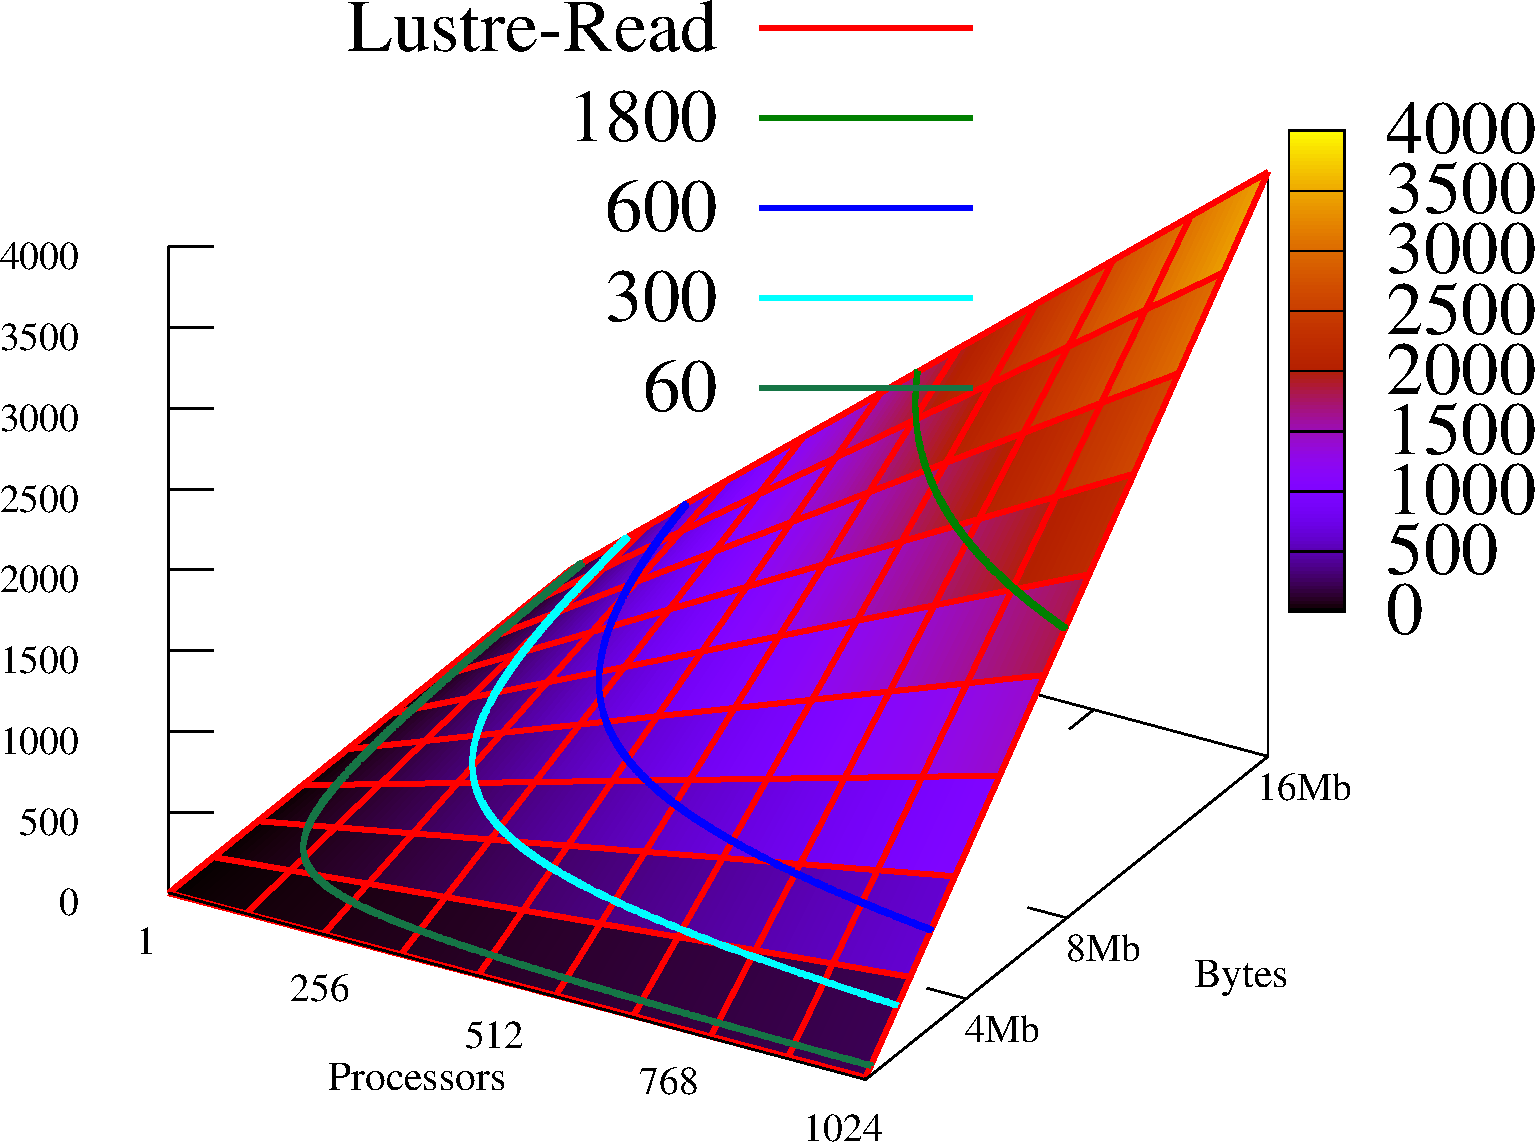
\includegraphics[width=\linewidth]{images/io/lustre-read}
%   \caption{Best case read performance with Lustre.}
%   \label{fig:lustre-read}
% \end{figure}
%
% \todo{repeat the same logic, except instead of reading
% `y' data, read $\frac{y}{16}$ data 16 times... as a
% really stupid unbricked app would do.}

% Compare this situation to application-level input: the
% program could easily be written to have process 0 open
% and read the desired data, and then send out the data
% to the processes which need it.  This would incur:
% \begin{eqnarray*}
%   T(N, b) &=& {} + 0.6 \mu{}s + (N \times 0.3 \mu{}s) \\
%           &&  {} + 9ms \\
%           &&  {} + (9ms + 4.2ms + (N \times b/102400)) \\
%           &&  {} + 2N \times (0.3 \mu{}s + 0.2 b \times 1024)
% \end{eqnarray*}
%
% Now only one process contacts the MDS; accordingly,
% the request and return are only paid once. Process 0
% still must send N requests for data, however. Seeking
% on the MDS is unchanged: we only looked for one file
% in the first place anyway. We avoid all but one of the
% seek costs on the OST
% BLAH -- the above is wrong, the file will be striped
% across multiple OSTs. Need to fix the case before
% this too.

% \note{Verified on Lens and Longhorn: the default
% stripe count in Lustre is 4, and the default stripe
% size is 1 megabyte. This is probably pretty terrible
% for performance. We should incorporate this info into
% the text, somehow...}

% \todo{Can we write a UVF multiple ways to demonstrate the importance
% of matching stripe size?  For example, if each brick in a UVF is
% 16 megabytes, and we make a stripe 16 megabytes... will we get bad
% performance because the 100-or-so byte header offsets everything
% poorly?  If we write the header to a separate file, does that improve
% our performance?}

% \todo{Or maybe somehow simulate same using `dd'...}

% \note{see \url{http://www.nics.tennessee.edu/io-tips}}
